\documentclass{article}
\usepackage{graphicx}

\title{Computer}
\author{Wikipedia}

\date{\today}
\renewcommand*\contentsname{Summary}

\begin{document}


\maketitle
\newpage
\tableofcontents

\section{Etymology}
\begin{figure}

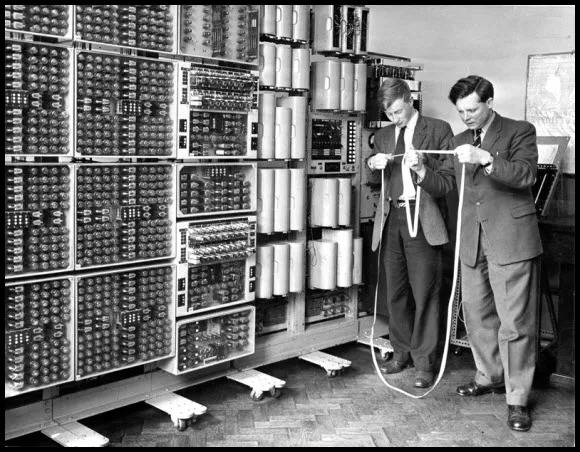
\includegraphics[width=\linewidth]{comp.jpg}

\caption{A boat.}

\label{fig:boatI}

\end{figure}

Figure \ref{fig:boatI} shows a boat\\

This is the first section.

According to the Oxford English Dictionary, the first known use of computer was in a 1613 book called The Yong Mans Gleanings by the English writer Richard Brathwait: "I haue [sic] read the truest computer of Times, and the best Arithmetician that euer [sic] breathed, and he reduceth thy dayes into a short number." This usage of the term referred to a human computer, a person who carried out calculations or computations. The word continued with the same meaning until the middle of the 20th century. During the latter part of this period women were often hired as computers because they could be paid less than their male counterparts.[1] By 1943, most human computers were women.[2]


The Online Etymology Dictionary gives the first attested use of computer in the 1640s, meaning 'one who calculates'; this is an "agent noun from compute (v.)". The Online Etymology Dictionary states that the use of the term to mean "'calculating machine' (of any type) is from 1897." The Online Etymology Dictionary indicates that the "modern use" of the term, to mean 'programmable digital electronic computer' dates from "1945 under this name; [in a] theoretical [sense] from 1937, as Turing machine".[3]

\section{History}
This is the second section

\subsection{Pre-20th century}

Devices have been used to aid computation for thousands of years, mostly using one-to-one correspondence with fingers. The earliest counting device was most likely a form of tally stick. Later record keeping aids throughout the Fertile Crescent included calculi (clay spheres, cones, etc.) which represented counts of items, likely livestock or grains, sealed in hollow unbaked clay containers.[a][4] The use of counting rods is one example.

\subsection{First computer}
Charles Babbage, an English mechanical engineer and polymath, originated the concept of a programmable computer. Considered the "father of the computer",[17] he conceptualized and invented the first mechanical computer in the early 19th century. After working on his revolutionary difference engine, designed to aid in navigational calculations, in 1833 he realized that a much more general design, an Analytical Engine, was possible. The input of programs and data was to be provided to the machine via punched cards, a method being used at the time to direct mechanical looms such as the Jacquard loom. For output, the machine would have a printer, a curve plotter and a bell. The machine would also be able to punch numbers onto cards to be read in later. The Engine incorporated an arithmetic logic unit, control flow in the form of conditional branching and loops, and integrated memory, making it the first design for a general-purpose computer that could be described in modern terms as Turing-complete.[18][19]

\end{document}